\documentclass{acmsiggraph}                     % final
%\documentclass[annualconference]{acmsiggraph}  % final (annual conference)
%\documentclass[review]{acmsiggraph}            % review
%\documentclass[widereview]{acmsiggraph}        % wide-spaced review
%\documentclass[preprint]{acmsiggraph}          % preprint

%% Uncomment one of the five lines above depending on where your paper is
%% in the conference process. ``review'' and ``widereview'' are for review
%% submission, ``preprint'' is for pre-publication, and ``final'' is for
%% the version to be printed. The ``final'' variant will accept the 
%% ``annualconference'' parameter, which changes the height of the space
%% left clear for the ACM copyright information.

%% The 'helvet' and 'times' packages define the typefaces used for
%% serif and sans serif type in this document. Computer Modern Roman 
%% is used for mathematics typesetting. The scale factor is set to .92
%% to bring the sans-serif type in line with the serif type.

\usepackage[scaled=.92]{helvet}
\usepackage{times}

%% The 'graphicx' package allows for the inclusion of EPS figures.

\usepackage{graphicx}

%% use this for zero \parindent and non-zero \parskip, intelligently.

\usepackage{parskip}

%% Optional: the 'caption' package provides a nicer-looking replacement
%% for the standard caption environment. With 'labelfont=bf,'textfont=it',
%% caption labels are bold and caption text is italic.

\usepackage[labelfont=bf,textfont=it]{caption}

% Additional packages for our paper
\usepackage{subfigure}
\usepackage{listings}
\usepackage[usenames,dvipsnames]{color}
\lstset{
    language=C++,
    basicstyle=\small\ttfamily\bfseries,
    frame=tb,
    numbers=left,
    numberstyle=\tiny,
    numbersep=-4pt,
    columns=fullflexible,
    showstringspaces=false,
    captionpos=b,
    keywordstyle=\color{Blue},
    morekeywords={float3,uint32_t,ushort2},
    commentstyle=\color{OliveGreen},
    stringstyle=\color{BrickRed}
}

%% If you are submitting a paper to the annual conference, please replace 
%% the value ``0'' below with the numeric value of your OnlineID. 
%% If you are not submitting this paper to the annual conference, 
%% you may safely leave it at ``0'' -- it will not be included in the output.

\onlineid{0}

%% Paper title.

\title{Haste: A Highly Parallel CUDA Monte Carlo Ray Tracer}

%% Author and Affiliation (single author).

%%\author{Roy G. Biv\thanks{e-mail: roy.g.biv@aol.com}\\Allied Widgets Research}

%% Author and Affiliation (multiple authors).

\author{Bob Somers \thanks{e-mail: rsomers@calpoly.edu} \\ Computer Science Dept. \\ College of Engineering \\ California Polytechnic State University %
\and Chris Gibson \thanks{e-mail: cgibson@calpoly.edu} \\ Computer Science Dept. \\ College of Engineering \\ California Polytechnic State University}

%% Keywords that describe your work.

\keywords{ray tracing, GPGPU, Monte Carlo rendering}

%%%%%% START OF THE PAPER %%%%%%

\begin{document}

\teaser{
    \subfigure{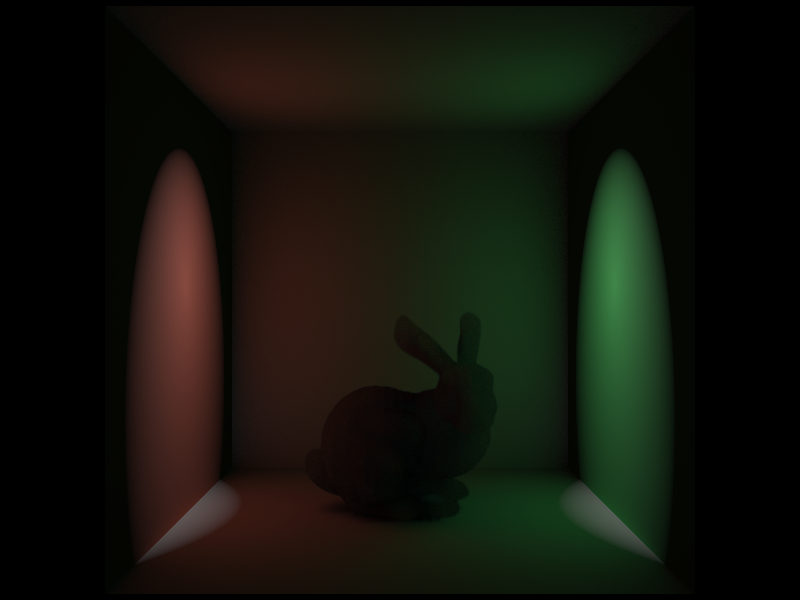
\includegraphics[height=1.5in]{img/two_light_bunny_indir.png}}
    \subfigure{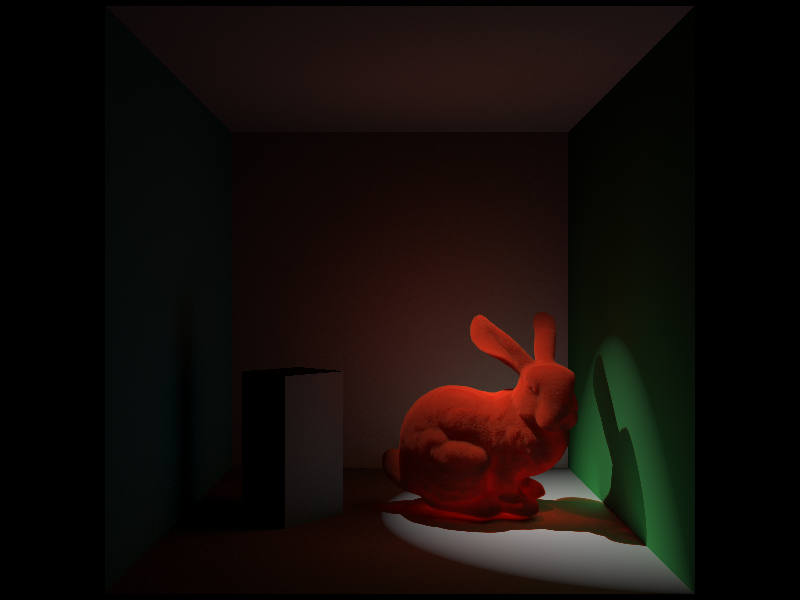
\includegraphics[height=1.5in]{img/ketchup_good.png}}
    \subfigure{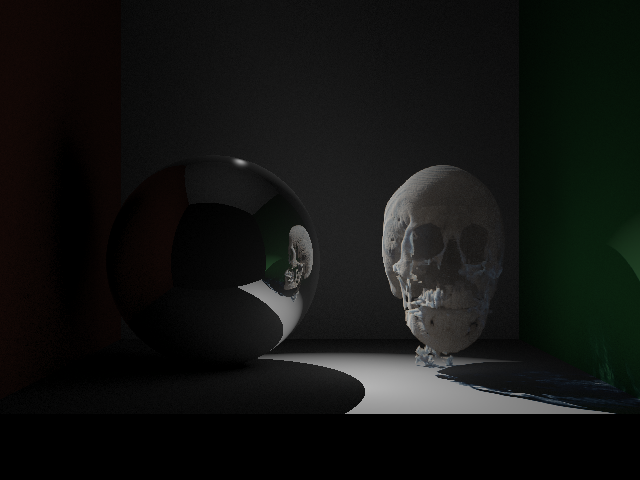
\includegraphics[height=1.5in]{img/sphere_skull.png}}
}

%% The ``\maketitle'' command must be the first command after the
%% ``\begin{document}'' command. It prepares and prints the title block.

\maketitle

%% Abstract section.

\begin{abstract}

We implement and evaluate a full Monte Carlo GPU-based renderer using CUDA, demonstrating the vast
improvements gained when running naturally parallel processes such as ray tracing and shading on
the Tesla series NVIDIA GPUs. We explain how our implementation builds off of existing algorithms,
but goes beyond na\"{i}ve single-bounce rendering and achieves a high level of parallelism despite
its recursive nature. We go into detail where the CPU's responsibilities end and where
the GPU's begin. We explain the bugs we ran into, the lessons learned during the design process,
and where this project is expected to go next.

\end{abstract}

%% ACM Computing Review (CR) categories. 
%% See <http://www.acm.org/class/1998/> for details.
%% The ``\CRcat'' command takes four arguments.

\begin{CRcatlist}
    \CRcat{I.3.7}{Computer Graphics}{Three-Dimensional Graphics and Realism}{Raytracing}
    \CRcat{I.3.1}{Computer Graphics}{Hardware Architecture}{Parallel Processing}
    \CRcat{I.6.8}{Simulation and Modeling}{Types of Simulation}{Monte Carlo}
\end{CRcatlist}

%% The ``\keywordlist'' command prints out the keywords.
\keywordlist

\section{Introduction}
\label{sec:intro}

    Ray tracing is a common technique for generating images based on a three-dimensional scene by 
    tracing the path of light through pixels on a user-defined plane (such as an image plane 
    defined by camera basis vectors). This technique is capable of a high level of realism, while 
    remaining reasonably efficient.

    By design, every ray sent out in the initial ray cast is independent. That ray may intersect 
    with objects in a scene, cast out rays in order to determine the shading state, and recurse as 
    the light is reflected or refracted through the objects in the scene that it hits. (Figure
    \ref{fig:diagram})
    
    \begin{figure}[htb]
        \begin{center}
            \leavevmode
            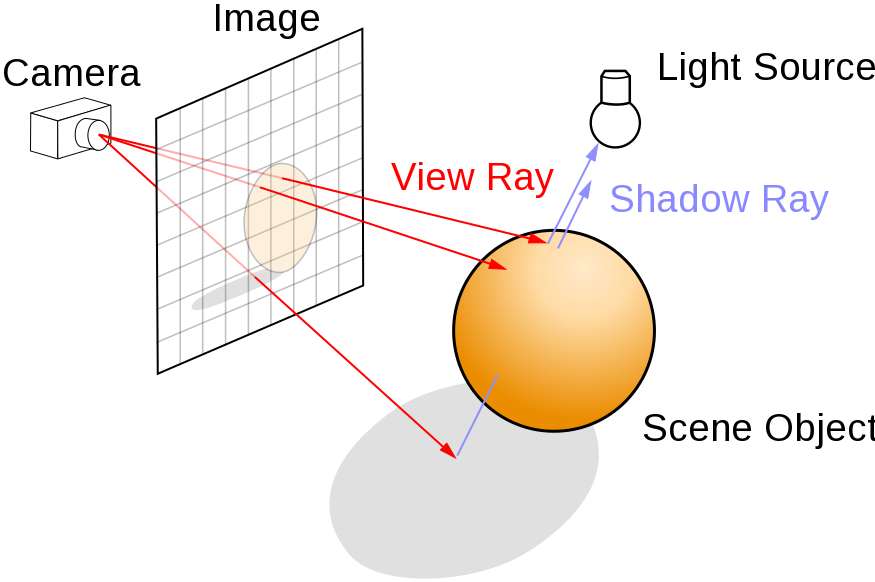
\includegraphics[width=2.5in]{diagram.png}
        \end{center}
        \caption{Ray tracing involves casting rays out of the eye, computing object intersections,
            and shading those points with respect to the lights.}
        \label{fig:diagram}
    \end{figure}

    Ray tracing, at its core, is an approximation of how rays of light would behave in reality.
    There are, however, many drawbacks to typical Whitted ray tracing. First off, the rays 
    cast to check if a particular point is in shadow or not take a very na\"{i}ve approach 
    to shading. The diffuse value of the light is either applied or it is not. Additionally,
    indirect light and caustics are not taken into account, which contributes a large majority
    of light in reality.

    The Monte Carlo method of ray tracing involves taking a sufficient number of random samples 
    in order to statistically estimate the the amount of light at any given point. This is broken
    into two parts, the direct light and indirect light contributions as opposed to the traditional
    model which simply sets a base ambient value.

    With recent advances in computing, particularly in GPU hardware, many have sought 
    to take advantage of the high degree of parallelism that such architectures offer. 
    Enter CUDA, a framework developed by NVIDIA for their next-generation GPUs.

    CUDA allows developers to take advantage of the hundreds of cores available in their graphics 
    cards with standard C code. This amount of parallelism is highly useful for a variety of
    applications such as physical simulations, graphics, financial estimation models, and video
    encoding to name a few.  As long as the algorithm can be broken down into smaller, iterative
    units, it can take advantage of the CUDA framework.

    In this paper, we show how our implementation takes the common recursive approach to Monte Carlo
    ray tracing and turns it into an iterative one for CUDA. Generalizing the ray casting algorithm
    so that all rays are treated the same (be they reflected, refracted or shading rays) allows us
    to implement a flexible framework in CUDA to intersect and shade all rays cast into a scene.

    The technique that we present is similar to the layer based approach first mentioned 
    in \cite{Segovia09}, but with additional improvements to make it more flexible. Specifically, we 
    show that storing more information with each ray (such as contribution factor, and its destination
    pixel and layer) allows us to avoid large memory-hungry ray batching and treats all rays equally,
    simplifying the implementation significantly.

\section{Related Work}
\label{sec:related}

Ray tracing on the GPU has been an area of heavy research recently, with work similar to ours, but with
some minor variations. Most implementations have made drastic assumptions about particular parts of the
rendering process, such as avoiding ray bouncing (ignoring the recursion problem) or avoiding Monte Carlo
(ignoring the memory problem).

    \subsection{Seminal Work}
    \label{sec:seminal}

    Turner Whitted's research \cite{Whitted80} is considered to be the fundamental underpinnings of
    ray tracing. Although the idea of casting rays from the eye into the scene was developed a few
    years earlier by Arthur Appel, Whitted was the first to follow this idea recursively, developing
    the basic algorithms that allow us to do reflection, refraction, and shadows with ray tracing.
    (Figure \ref{fig:whitted})

    \begin{figure}[htb]
        \begin{center}
            \leavevmode
            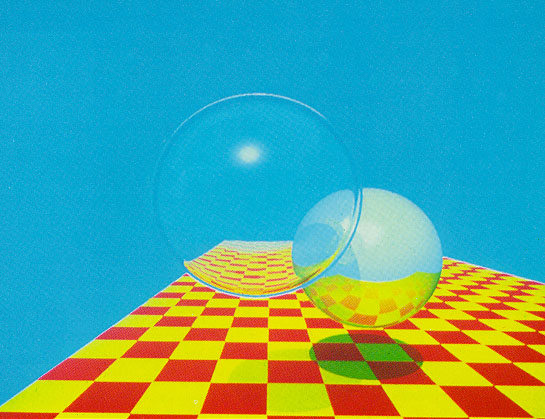
\includegraphics[width=2.5in]{whitted.jpg}
        \end{center}
        \caption{Whitted's renders were the first to demonstrate reflection, refraction, and shadows.}
        \label{fig:whitted}
    \end{figure}

    \subsection{Iterative Layer-Based Approach}
    \label{sec:layerbased}

    A significant hurdle in this project was rewriting the traditional ray tracing algorithm to
    be iterative. An iterative, layer-based approach is presented in \cite{Segovia09} that shows
    how one of the most difficult problems with rewriting the algorithm can be avoided using a
    stack of image buffers for each level of recursion.

    In sections \ref{sec:recursion} and \ref{sec:raystate}, we explore the parts of their work that apply to Haste, as
    well as the adjustments we made to enhance the flexibility of their approach.

    \subsection{NVIDIA OptiX}
    \label{sec:optix}

    OptiX is a generic ray tracing engine built using CUDA for NVIDIA's GeForce and Tesla
    series GPUs. OptiX was designed to be as generic and flexible as possible, to accelerate
    the task of casting rays for a variety of scientific purposes, not just image rendering. Using
    OptiX involves writing subprograms to test intersections of objects in the scene, as well
    as compute shading values (if desired) when intersections occur. \cite{Parker10}

\section{Lighting Model}
\label{sec:lighting}

Before we could begin porting the ray tracing algorithm to CUDA, we needed to
nail down exactly how we were going to compute shading for the objects in the
scene. For Haste, we opted to go with the Phong lighting model, which we were
both familiar with. The Phong model attempts to capture the way light interacts
with a surface by breaking it up into three distinct components.

\begin{itemize}
    \item The \textbf{ambient} component is light that reaches the surface by
    being reflected off of other objects in the environment. In real-time pipelines,
    this is usually a constant flat color and is somewhat of a hack.

    \item The \textbf{diffuse} component is light that reaches the surface directly
    from a light and then is scattered in many directions due to the surface's microscopic roughness.
    This is the primary contributor for most objects.

    \item The \textbf{specular} component is light that reaches the surface directly
    from a light and then reflects around the same angle due to the surface's
    smoothness. It is typically identified as a "shiny spot", and is dependent on the
    viewer's location relative to the object and the light.
\end{itemize}

In addition to these three, there is one additional contributor that is typically
left out of the Phong equation in real-time pipelines.

\begin{itemize}
    \item The \textbf{emissive} component is light that is emitted by the surface
    itself rather than reflected from other lights or the environment.
\end{itemize}

While most real-time pipelines ignore this term since lights and objects are handled
separately, our global illumination approach requires us to consider this term as well.
In fact, Haste makes no distictions between lights and objects. Lights are simply objects
with an emissive component greater than zero.

Thus, our lighting equation, shown in (\ref{eq:illumination}), determines the illumination
(color) $I$ at a point $p$ on the surface of an object.

\begin{equation}
    \label{eq:illumination}
    I_{p} = E_{p} + A_{p} + D_{p} + S_{p}
\end{equation}

Where $E_{p}$, $A_{p}$, $D_{p}$, and $S_{p}$ are the emissive, ambient, diffuse, and
specular components respectively.

    \subsection{Diffuse Lighting}
    \label{sec:diffuse}
    
    The diffuse component, shown in (\ref{eq:diffuse}), is a sum of all the contributions
    from each light $m$. Each light's contribution is function of the surface's diffuse
    reflection constant $k_{d}$, the direction vector $\vec{L_{m}}$ from $p$ to the light,
    the normal vector $\vec{N}$ of the surface at $p$, and the diffuse color $i_{d}$ of the
    surface and the light.

    \begin{equation}
        \label{eq:diffuse}
        D_{p} = \sum_{m \textrm{ } \in \textrm{\small{ lights}}}^{}
            k_{d} \left( \vec{L_{m}} \cdot \vec{N} \right) i_{d}
    \end{equation}

    \subsection{Specular Lighting}
    \label{sec:specular}

    Similarly, the specular component, shown in (\ref{eq:specular}), is a sum of all the
    contributions from each light $m$. Each light's contribution is a function of the
    surface's specular reflection constant $k_{s}$, the reflection vector $\vec{R_{m}}$
    of the light vector about the surface normal at $p$, the view vector $\vec{V}$ from
    the $p$ to the viewer, the specular power $\alpha$ (shininess), and the specular
    color $i_{s}$ of the light.

    \begin{equation}
        \label{eq:specular}
        S_{p} = \sum_{m \textrm{ } \in \textrm{\small{ lights}}}^{}
            k_{s} \left( \vec{R_{m}} \cdot \vec{V} \right) ^{\alpha} i_{s} 
    \end{equation}

    \subsection{Monte Carlo}
    \label{sec:montecarlo}

    The problem with (\ref{eq:diffuse}) and (\ref{eq:specular}) is that if we only take one
    sample per light, we treat our lights as point lights instead of area lights. This causes
    us to lose our soft phenomena, such as soft shadows. In reality, $p$ may be able to see
    part of the light, while some of the light is obscured.
    
    To simulate this, we use a Monte Carlo approach and uniformly sample across the volume
    of the light. For each sample $j$ in $n$ samples, we generate a random point $p_{L}$
    inside the volume of the light and use that point to calculate the light direction vector
    $L_{m}$. This leads to the following adjustments to (\ref{eq:diffuse}) and
    (\ref{eq:specular}) respectively:

    \begin{equation}
        \label{eq:diffuse_mc}
        D_{p} = \sum_{m \textrm{ } \in \textrm{\small{ lights}}}^{} \left[
            \sum_{j = 1}^{n} \frac{1}{n} \textrm{ }
                k_{d} \left( \vec{L_{m}} \left( p_{L} \right) \cdot \vec{N} \right) i_{d}
        \right]
    \end{equation}

    \begin{equation}
        \label{eq:specular_mc}
        S_{p} = \sum_{m \textrm{ } \in \textrm{\small{ lights}}}^{} \left[
            \sum_{j = 1}^{n} \frac{1}{n} \textrm{ }
                k_{s} \left( \vec{R_{m}} \left( p_{L} \right) \cdot \vec{V} \right) ^{\alpha} i_{s}
        \right]
    \end{equation}

    \subsection{Ambient Lighting}
    \label{sec:ambient}

    As mentioned above, in real-time graphics pipelines the ambient term is somewhat of
    a hack. It's flat color value is usually used to prevent an object from fading completely
    to black in areas where its diffuse contribution is small. The constant flat
    color is a local approximation of what actual ambient lighting would contribute.

    However, in a global illumination system (such as Haste), we are not concerned with
    real-time performance, but rather rendering accuracy. Thus, we can accurately compute
    the ambient contribution, again using a Monte Carlo approach.

    The ambient component, shown in (\ref{eq:ambient_mc}), is a sum of all the contributions
    of each ambient sample taken. For each ambient sample, we generate a random ray in the
    hemisphere normal to $p$ and find the closest object it intersects with. We call this point
    $p_{A}$. For that point, we compute the simple (non-Monte Carlo) diffuse and specular
    lighting at that point, $D_{p_{A}}$ and $S_{p_{A}}$, explained in (\ref{eq:diffuse}) and
    (\ref{eq:specular}). In addition, each ambient sample relies on the surface's ambient
    reflection constant $k_{s}$.

    \begin{equation}
        \label{eq:ambient_mc}
        A_{p} = \sum_{j = 1}^{n} \frac{1}{n} \textrm{ }
            k_{a} \left( D_{p_{A}} + S_{p_{A}} \right)
    \end{equation}
    
    \subsection{Emissive Lighting}
    \label{sec:emissive}

    Lastly, the emissive component, shown in (\ref{eq:emissive}) is rather straightforward.
    It simply consists of the surface's emissive constant $k_{e}$ and the emissive color
    $i_{e}$ of the surface. There is no need to sample this component with a Monte Carlo
    approach.

    \begin{equation}
        \label{eq:emissive}
        E_{p} = k_{e} \textrm{ } i_{e}
    \end{equation}

\section{Parallelizing the Algorithm}
\label{sec:parallelalgo}

Graphics in general, especially ray tracing, is one of the classic problems that is
said to be ``embarassingly parallel". We quickly found, however, that this is usually
touted by people who have never attempted to implement a highly parallelized ray
tracer. While the problem indeed has an enormous amount of exploitable data-level
parallelism, there are significant hurdles in rewriting the algorithm itself to work
on highly parallel hardware, such as NVIDIA's CUDA platform.

    \subsection{Eliminating Recursion}
    \label{sec:recursion}

    The crux of the problem is that the traditional ray tracing algorithm itself is
    recursive, with successively bounced rays contributing color in a cumulative fashion.
    Color is summed from the furthest bounce inwards for each pixel as rays are
    successively popped off the stack, like so:
    
    \begin{equation}
        \label{eq:recursive_sum}
        \textrm{pixel} = \textrm{ray}_{0} \cdot R_{0} \left( \textrm{ray}_{1} \cdot R_{1}
            \left( \textrm{ray}_{2} \ldots R_{n - 1} \left( \textrm{ray}_{n} \right) \right)
        \right)
    \end{equation}

    where $R_{n - 1}$ is the fraction of light from $\textrm{ray}_{n - 1}$ that was bounced
    in the direction of $\textrm{ray}_{n}$. 
    
    CUDA, at this time, does not have support for recursive function calls. Thus, the
    algorithm needed to be rewritten iteratively. However, this must be done carefully, because
    na\"{i}vely refactoring the standard ray tracing algorithm does not take this recursive
    summing into account.

    \cite{Segovia09} presents an interesting approach which uses a series of
    layer buffers to effectively give you a stack of final image buffers. The rays are traced
    in ``batches", where each new batch draws into the next layer buffer down. The layer buffers
    are then summed in a weighted fashion such that the final sum matches the recursive approach.
    
    Our approach is similar, but with some minor modifications. The Segovia approach is limited
    because all objects in the scene have the same $R_{n}$, since the layers are summed after
    the fact. In Haste, the rays themselves contain additional state, discussed in more detail
    in section \ref{sec:raystate}.
    
    One of those pieces of state is the ray's ``contribution factor", which is multiplied against
    all shading calculations for that ray. When a ray spawns a reflected or refracted ray, the
    new ray has its contribution factor set to that of its parent, multiplied by the reflection
    or refraction constant for that surface, like so:

    \begin{equation}
        C_{n} = C_{n - 1} \cdot R_{n - 1}
    \end{equation}

    where $C_{n}$ is the contribution factor for $\textrm{ray}_{n}$. 

    with this modification, the correct color summing is performed on a per-object basis rather
    than a per-layer one. Thus, the layers should be summed using a flat sum instead of the weighted
    sum used in the Segovia approach.

    \subsection{Streaming Stateful Rays}
    \label{sec:raystate}

    In \cite{Segovia09}, rays are traced in batches, with each batch
    corresponding to a new layer of ``recursion". Since Haste uses a Monte Carlo method for
    rendering, it is definitely conceiveable that the number of rays in successive layers could
    grow wildly out of control, potentially using up all available memory on the GPU.
    
    To combat this, we encode additional state information in each ray so that it knows exactly
    what pixel and layer it contributes to. This allows us to trace rays in arbitrary batch sizes
    to tune for memory efficiency as well as kernel launch size. With one thread allocated per
    ray, our additional state allows us cast more total rays than the maximum possible launch size.

    A structure to hold a typical stateless ray would look something like listing \ref{rayorig}.

    \begin{lstlisting}[caption=A traditional stateless ray structure.,label=rayorig]
    typedef struct Ray {
        float3 origin;
        float3 direction;
    } Ray;
    \end{lstlisting}

    Our new stateful ray structure stores additional information along with the origin and
    direction, as seen in listing \ref{raynew}.

    \begin{lstlisting}[caption=A stateful ray structure.,label=raynew]
    typedef struct Ray {
        float3 origin;
        float3 direction;
        float contrib; // contribution factor
        uint32_t layer; // contributing layer number
        ushort2 pixel; // contributing pixel coordinates
        bool unibounce; // single bounce ray?
    } Ray;
    \end{lstlisting}

    With this additional information, we are no longer dependent on tracing rays in batches
    per layer, nor are we limited to a constant $R_{n}$ for all objects. Each ray is
    independent and stores enough data to figure out which pixel and layer buffer to
    write its contribution into.

    This allows us to constantly stream input rays into the GPU and extract output rays (such
    as reflected and refracted rays) from the ray tracing kernel. The output rays are pushed
    into a ray queue that stores pending rays. When the GPU is ready for a kernel launch,
    we extract a packet of rays from the queue (one ray per GPU thread), copy the packet to
    the device, and launch the kernel. This process continues until the ray queue is depleted.

\section{Squashing Bugs}
\label{sec:bugs}

Many bugs arose during the development of Haste. Some were architectural, based 
on issues in our initial implementation decisions, while others were simply typos,
but were deviously hidden by the complexity of the system.

    \subsection{Normal Interpolation}
    \label{sec:normallerp} 

    \begin{figure}[htb]
        \begin{center}
            \leavevmode
            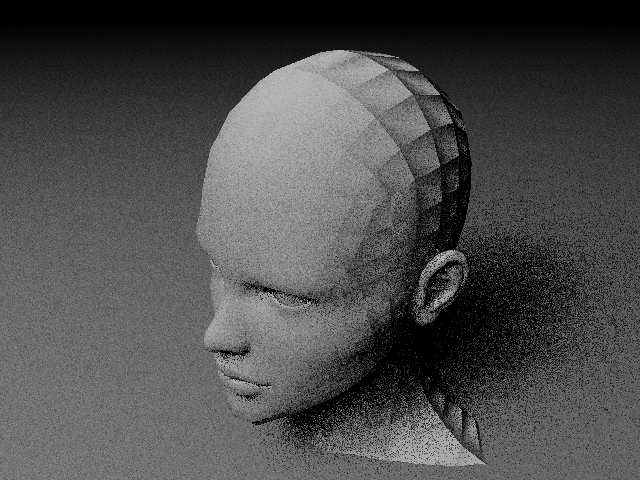
\includegraphics[width=2.5in]{badnormals.jpg}
        \end{center}
        \caption{Model with incorrectly interpolating normals.}
        \label{fig:bad_normals}
    \end{figure}

    One major bug that appeared turned out to be entirely unrelated to CUDA.  Although normal 
    interpolation within triangles seemed to work well, polygonal meshes (such as the Stanford bunny) would 
    show seams at the shared edges of triangles, as seen in Figure \ref{fig:bad_normals}.
    This lead to a thorough investigation with the assumption that the models were being loaded 
    incorrectly or that the normals were being modified incorrectly. The issue turned out to be 
    a simple arithmetic bug in the calculation of the interpolated normal. 

    \begin{figure}[htb]
        \begin{center}
            \leavevmode
            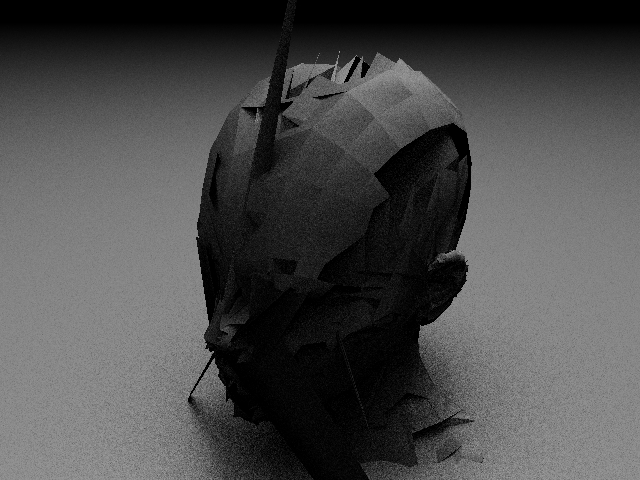
\includegraphics[width=2.5in]{ruinedhead.jpg}
        \end{center}
        \caption{Head model ruined by incorrect vertex parsing.}
        \label{fig:ruined_head}
    \end{figure}

    While investigating the normal interpolation bug, a modification to the normal and vertex 
    parsing code caused some rather unexpected results, as seen in Figure \ref{fig:ruined_head}.

    \subsection{Bounding Volume Hierarchy Traversal}
    \label{sec:bvhtraversal}

    There are many spatial data structures that can speed up intersection tests in a ray tracer.
    We chose to implement one of the most common, a bounding volume hierarchy (BVH). The basic idea is
    that objects in the scene are grouped into axis-aligned bounding boxes (AABBs) that are
    then grouped spatially in a binary tree structure (Figure \ref{fig:bvh}). Because of the spatial grouping, if a ray
    does not intersect a bounding box node in the tree, it is guaranteed to not intersect either
    of the two subtrees or any objects contained therein. Thus, we can reduce the number of
    intersection tests from $O\left(n\right)$ to $O\left(\log n\right)$.
   
    \begin{figure}[htb]
        \begin{center}
            \leavevmode
            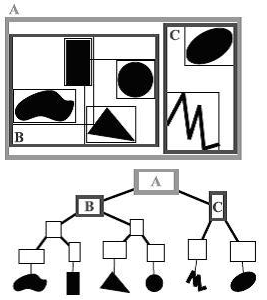
\includegraphics[width=2.5in]{bvh.png}
        \end{center}
        \caption{An example of a two-dimensional bounding volume hierarchy.}
        \label{fig:bvh}
    \end{figure}

    This is a big win for performance. For example, in a scene with 30k triangles, instead of
    testing each ray against all 30k objects we can reduce this down to roughly 16 intersection tests.
    The only downside is that the intersection test code becomes more branchy, which is bad
    for the CUDA architecture.

    A significant hurdle in implementing the traversal code is, not surprisingly, eliminating
    recursion. Traditionally both BVH construction and traversal algorithms are recursive.
    Refactoring them to do an interative traversal is not trivial, because it's not simply a
    matter of traversing the tree. Since the point of building the BVH is to selectively
    \emph{not} traverse large chunks of the tree, there is some logic at each node that needs
    to make decisions about where to head next based on the traversal history.

    Our first approach was stackless, and involved using parent pointers and a previous record
    to determine both the location in tree and where to head next. This code is still buggy,
    and at this point, will probably be scrapped.

    Since we know the depth of the tree at construction time (which happens on the CPU), we know
    how much memory to allocate for a traversal stack. We will likely refactor the traversal
    algoroithm to use a stack-based iterative traversal. This is a high priority item on
    our future work agenda.

\section{Results}
\label{sec:results}

Results can be viewed at the end of this paper.  Figures \ref{fig:spheres}, \ref{fig:skull} 
and \ref{fig:cartblue} are all pictures generated by our renderer.

\section{Future Work}
\label{sec:future}

Although we have generated some striking images, there is still much to be expanded on for
Haste to be considered complete. These include general improvements to the base code (which
will continue on the master branch) as well as specialized improvements for our Masters
theses (which will happen on separate branches).

    \subsection{General Improvements}
    \label{sec:generalimprove}

    Although making certain assumptions from the start helped us avoid many issues that na\"{i}ve 
    GPU ray tracers run into, many issues exist that will likely be improved in the near future.
    
    One example is the fact that the CUDA kernels are currently only supported by Fermi 
    architecture, which limits what hardware the software can run on. This is not a trivial issue,
    as some of our algorithms assume certain features and operations are available in the hardware
    when running. The most important operation we rely on is atomic addition of floating point 
    numbers, which is not available in pre-Fermi architecture GPUs.

    Additionally, our current method of transferring ray packets to and from the GPU is inefficient,
    reallocating the device-side memory for each packet sent. This can be very costly. An
    improvement beyond simply allocating device-side memory once would be to setting up CUDA streams,
    allowing the GPU to be performing three tasks at once: Pulling rays from the CPU,
    testing ray-object intersections and shading, and pushing intersections off the GPU.

    The CUDA kernel currently implemented is a one-kernel-fits-all direct-lighting shader. When more 
    complex scene objects (like volumes) come into play, this will not be a viable option. The
    intersections, shading and volume integration may all have to be split into separate kernels 
    in order to take full advantage of the SIMD architecture that CUDA offers.

    \subsection{Distributed Rendering of Massive Scenes}
    \label{sec:distributed}

    A current limitation of all GPU ray tracers is that all the scene geometry must fit into the
    GPU's memory. This is a severe limitation for adoption of GPU rendering in the entertainment
    industry, since it is not uncommon to render scenes with many large meshes, thousands of
    textures, and volumetric effects.

    Haste is highly parallel on a single machine, but we would like to extend it to be highly
    parallel across a cluster of machines. Specifically, we'd like to parallelize across the
    distribution of scene geometry, allowing a distributed version of Haste to render scenes too
    large to fit on a single machine.

    \subsection{High Performance Volume Rendering}
    \label{sec:volumes}

    Future improvements will include the generation, lighting, and rendering of volumetric data
    within scene files. Fluid and smoke simulations within the CUDA kernel will significantly
    speed up simulation times. Although parallel volume ray tracing is more complex due to its
    naturally large size requirements, there are many algorithms to help mitigate the memory 
    issues.

\section*{Acknowledgements}

We'd like to thank Dr. Zo\"{e} Wood for teaching the Advanced Rendering class and sparking
our interest in ray tracers. In addition, her constant prodding to stop building hacky
workarounds and go with a fully Monte Carlo solution was, as usual, right on target.

We'd also like to thank Dr. Chris Lupo for his ability to procure obscenely powerful
supercomputers for us to play around with, as well as his insightful lectures that always
seemed to end with the punchline: ``It depends".

\begin{figure*}[ht]
    \centering
    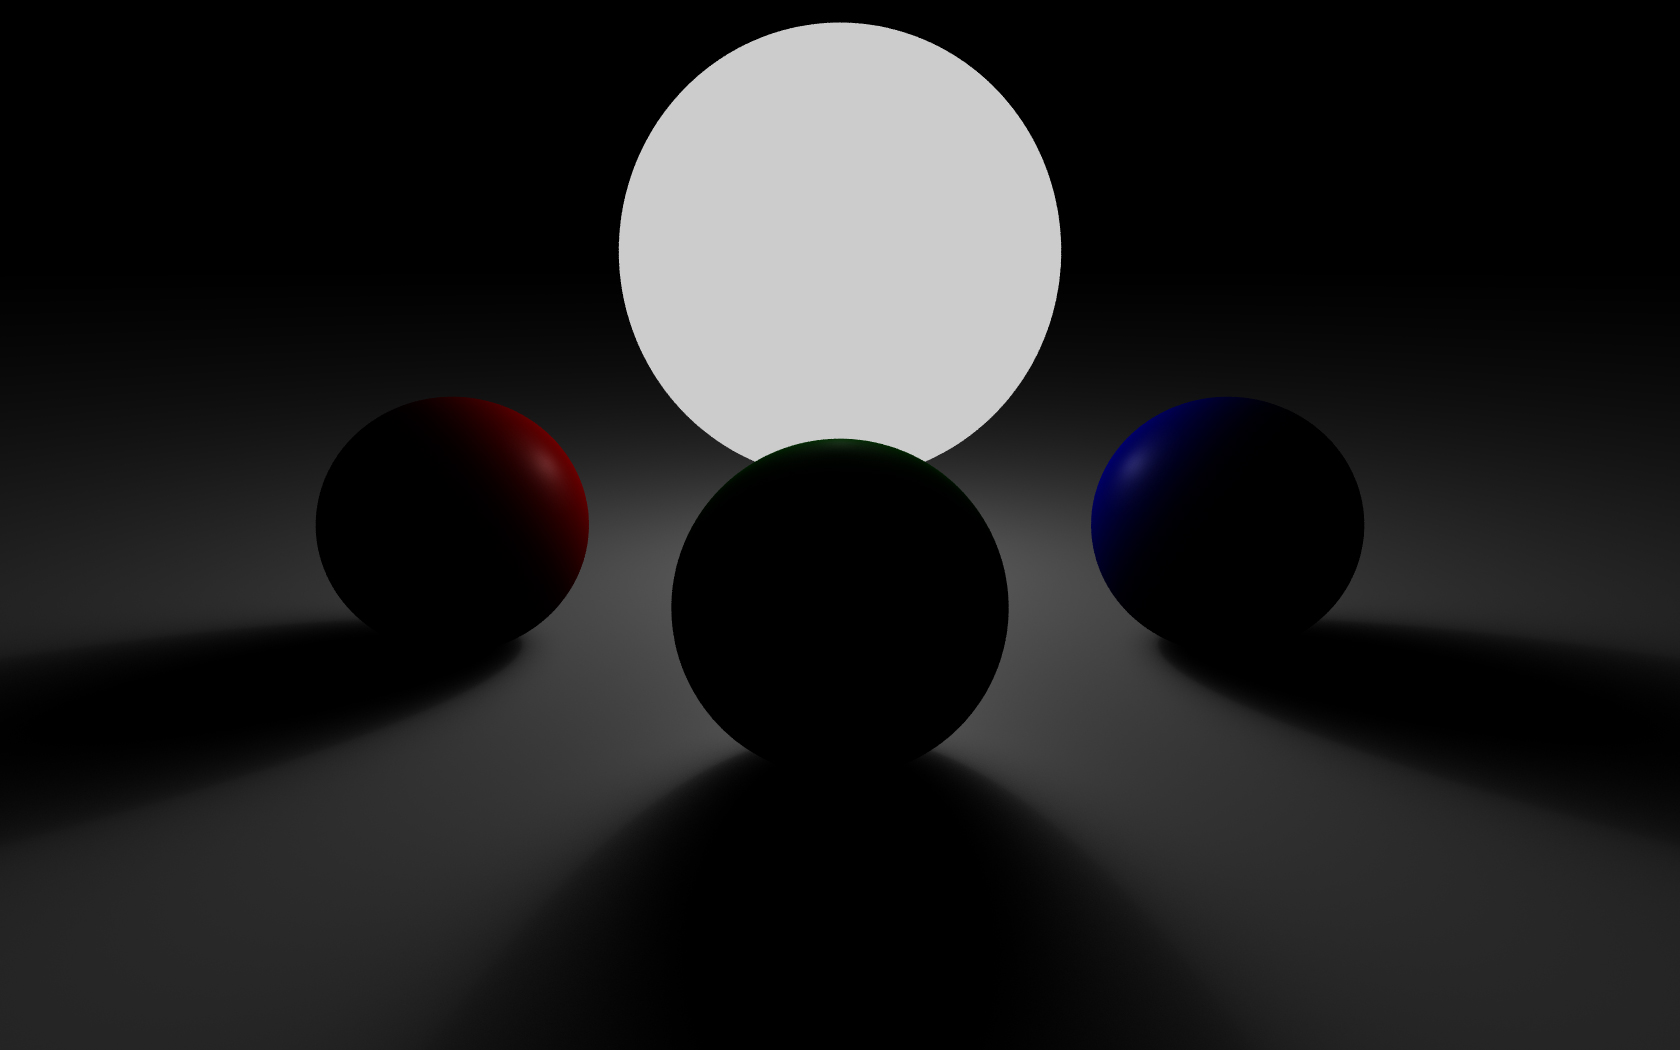
\includegraphics[width=6in]{spheres.jpg}
    \caption{Three spheres casting soft shadows from an area light.}
    \label{fig:spheres}
\end{figure*}

\begin{figure*}[ht]
    \centering
    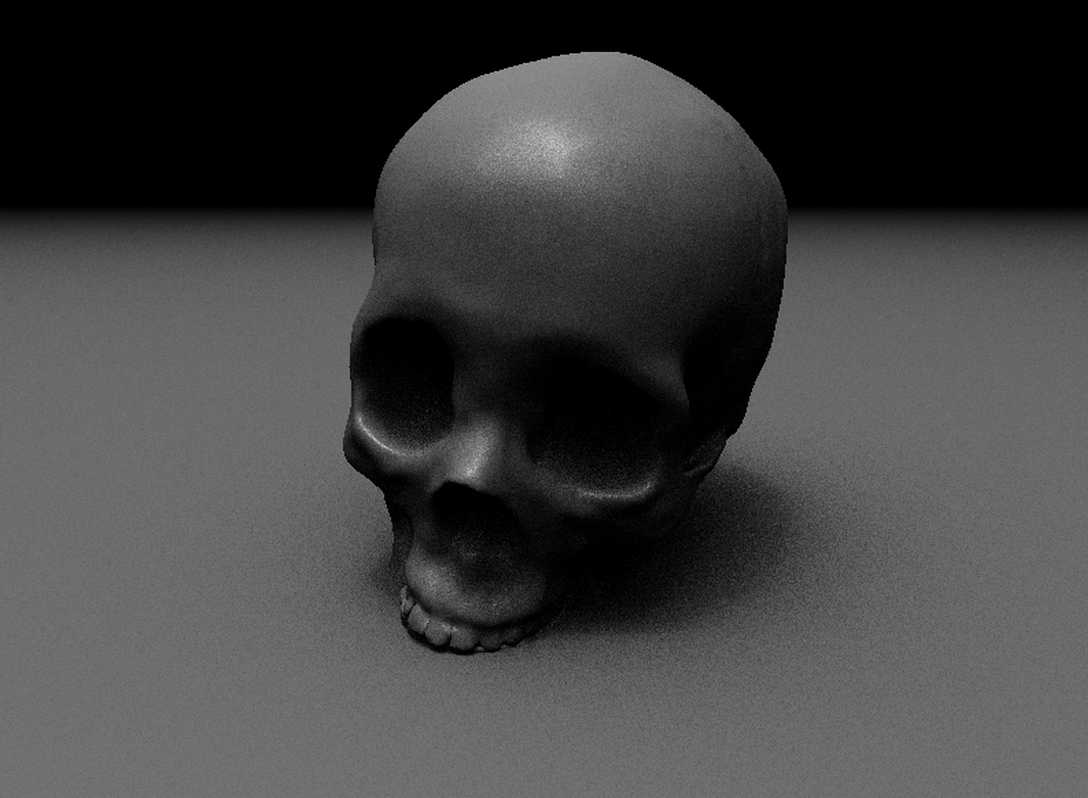
\includegraphics[width=6in]{skull.png}
    \caption{Skull model rendered with an area light.}
    \label{fig:skull}
\end{figure*}

\begin{figure*}[ht]
    \centering
    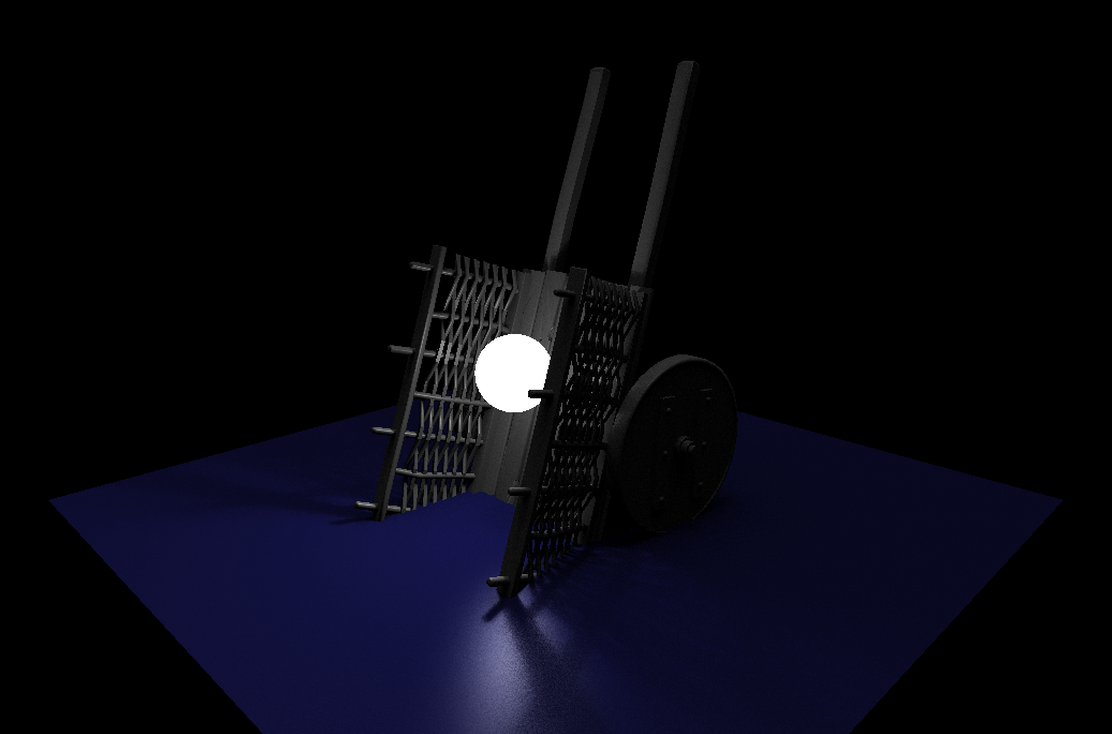
\includegraphics[width=6in]{cartblue.png}
    \caption{Cart model rendered showing the soft shadows cast with a small area light.}
    \label{fig:cartblue}
\end{figure*}

\bibliographystyle{acmsiggraph}
\nocite{*}
\bibliography{pbcbex}
\end{document}
